\documentclass{article}
\usepackage{iclr2026_conference}
\usepackage{hyperref}
\usepackage{graphicx}
\usepackage{amsmath}
\usepackage{amssymb}

\title{Integrating Text-Based Problem Descriptions with Data-driven PDE Solver}

\author{Anonymous Authors \\ Paper under double-blind review}

\begin{document}

\maketitle

\begin{abstract}
Partial differential equations (PDEs) are fundamental to modeling a wide range of physical phenomena, including fluid dynamics, heat transfer, and wave propagation. Traditional numerical methods for solving PDEs are computationally expensive and require careful problem-specific design. This work investigates a multimodal approach to PDE surrogate modeling by integrating natural language descriptions with numerical data. We extend a UNet-based architecture using text embeddings as conditioning signals. Experiments across multiple PDE datasets show that baseline UNet performs best, while naive text conditioning does not consistently improve performance. These results highlight challenges in multimodal integration.
\end{abstract}

\section{Introduction}

% (Paste your full introduction here — unchanged)

\section{Background and Motivation}

\subsection{Partial Differential Equations in Scientific Modeling}

% (Paste content)

\begin{figure}[t]
\centering
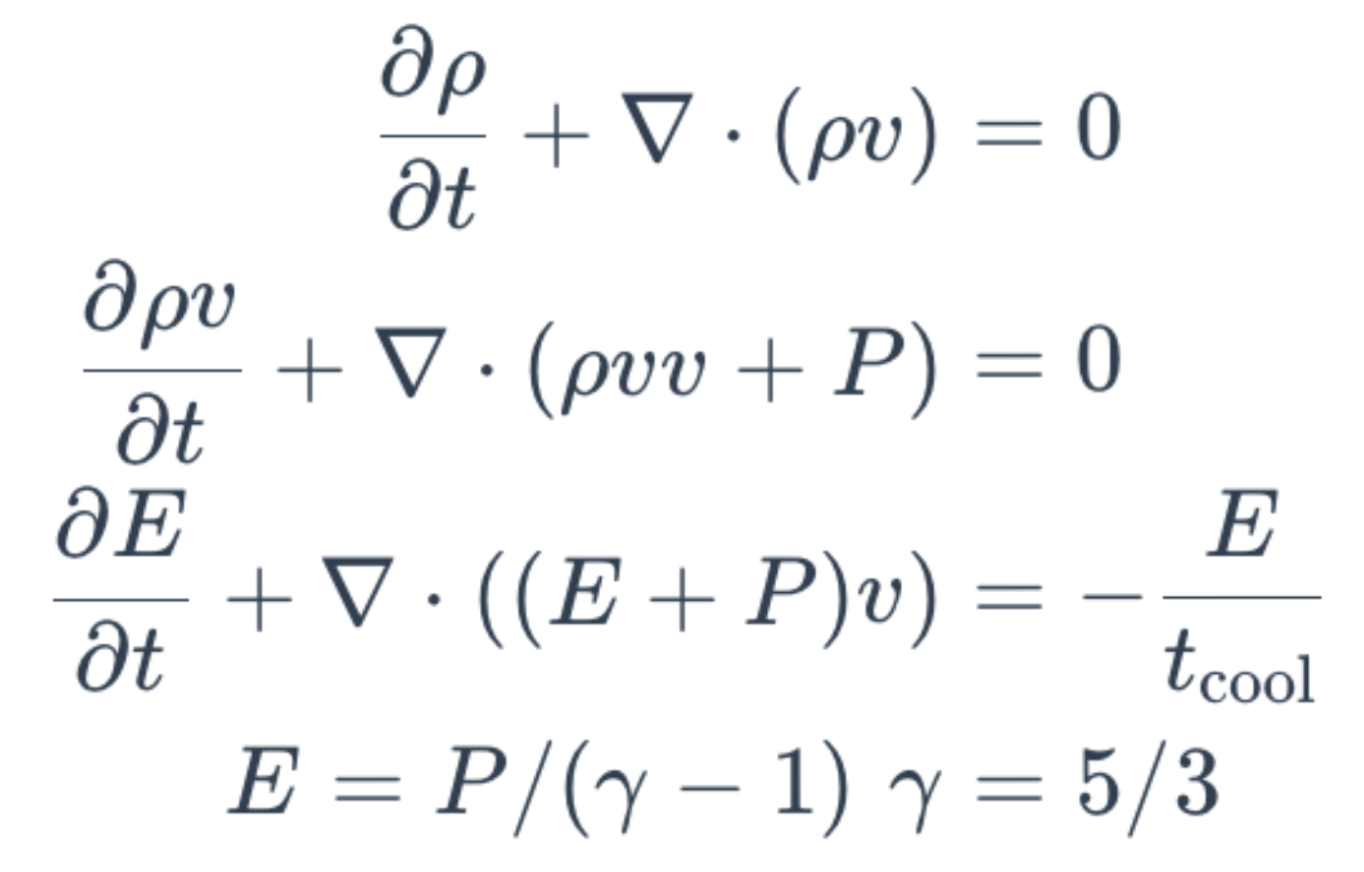
\includegraphics[width=0.9\columnwidth]{figures/turbulent_radiative_layer_2D.png}
\caption{Turbulent Radiative Layer 2D}
\label{fig:turbulent_radiative}
\end{figure}

\begin{figure}[t]
\centering

\includegraphics[width=0.9\columnwidth]{figures/active_matter_turbulent.png}
\caption{Active Matter and Turbulent Radiative Layer 2D}
\label{fig:active_matter_turbulent}
\end{figure}

\subsection{Data-Driven PDE Solvers}

% (Paste content)

\subsection{Generalization Challenges}

\begin{figure}[t]
\centering
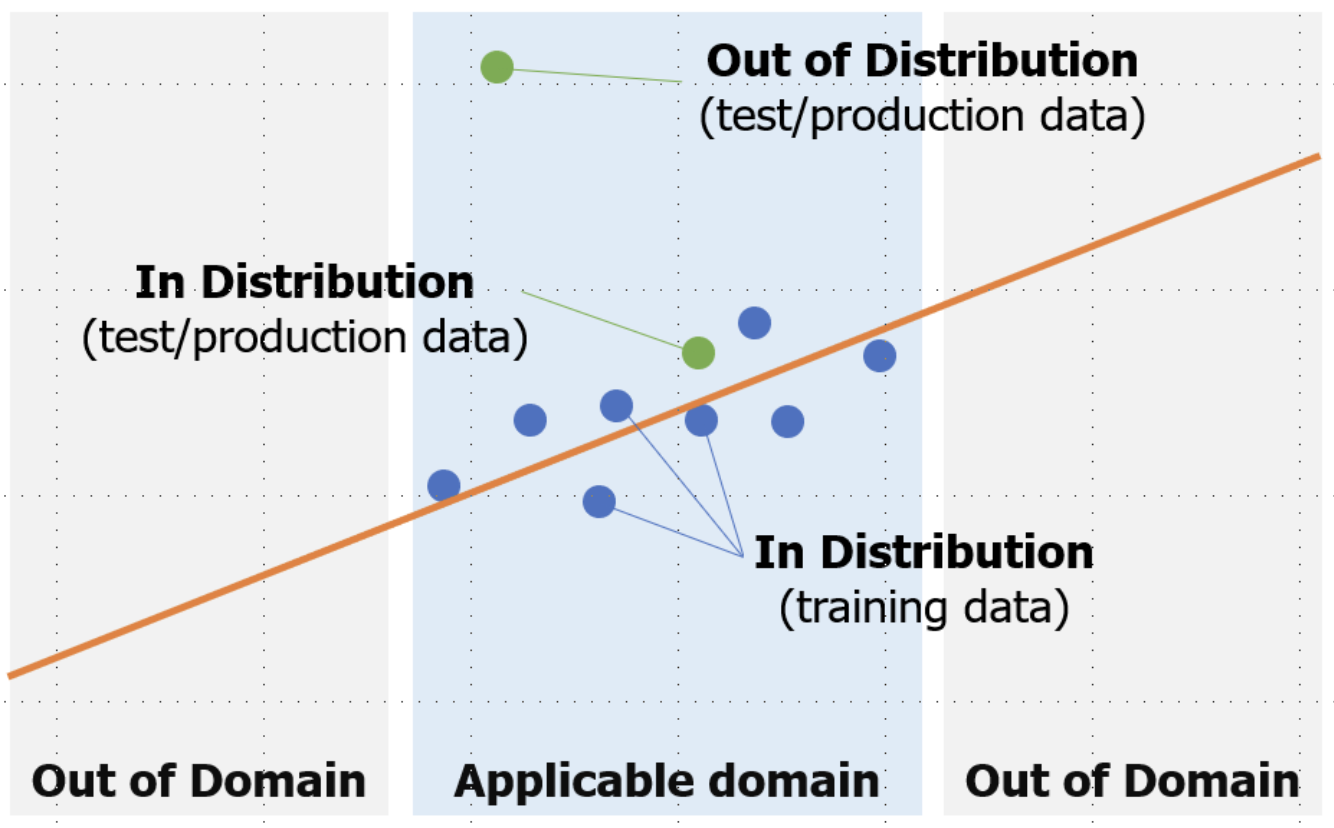
\includegraphics[width=0.9\columnwidth]{figures/ood_example.png}
\caption{Out-of-distribution scenarios}
\label{fig:ood}
\end{figure}

% (Continue content)

\section{Related Work}

% IMPORTANT: remove duplicate paragraphs you currently have

% (Paste cleaned related work)

\section{Methodology}

\subsection{Problem Formulation}

\begin{equation}
F(u, \nabla u, \nabla^2 u, x, t; \theta) = 0
\end{equation}

\begin{equation}
\hat{u}_{t+1} = f_\phi(u_{t-k:t}, C)
\end{equation}

\subsection{Data Representation}

\begin{equation}
X = [u_{t-3}, u_{t-2}, u_{t-1}, u_t]
\end{equation}

\subsection{Text-Based Conditioning}

\begin{equation}
c = W_2 \sigma(W_1 e + b_1) + b_2
\end{equation}

\subsection{UNet Architecture}

\begin{figure*}[t]
\centering
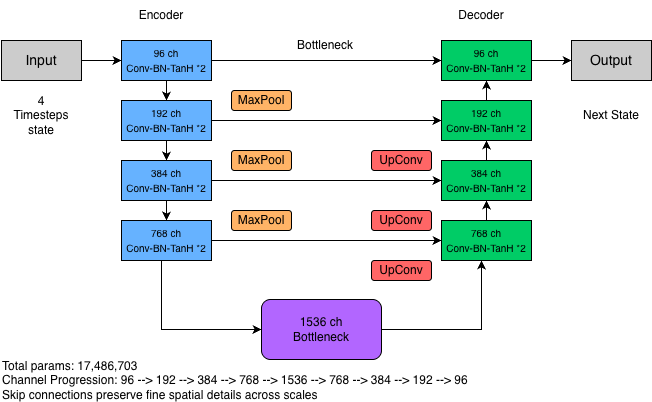
\includegraphics[width=\textwidth]{figures/unet_diagram.png}
\caption{UNet Architecture}
\label{fig:unet}
\end{figure*}

\subsection{Training Objective}

\begin{equation}
L_{\text{MSE}} = \frac{1}{N} \sum_{i=1}^N \|\hat{u}_i - u_i\|^2
\end{equation}

\begin{equation}
L_{\text{rollout}} = \sum_{t=1}^T \|\hat{u}_t - u_t\|
\end{equation}

\section{Experiments and Results}

\subsection{Overall Performance}

\begin{table}[t]
\centering
\caption{Rollout Test Loss}
\begin{tabular}{lc}
\hline
Model & Loss \\
\hline
UNetClassic & 0.13627 \\
UNetConditioned & 0.15746 \\
AViT (cond) & 0.48534 \\
AViT & 0.71870 \\
\hline
\end{tabular}
\end{table}

\begin{figure}[t]
\centering
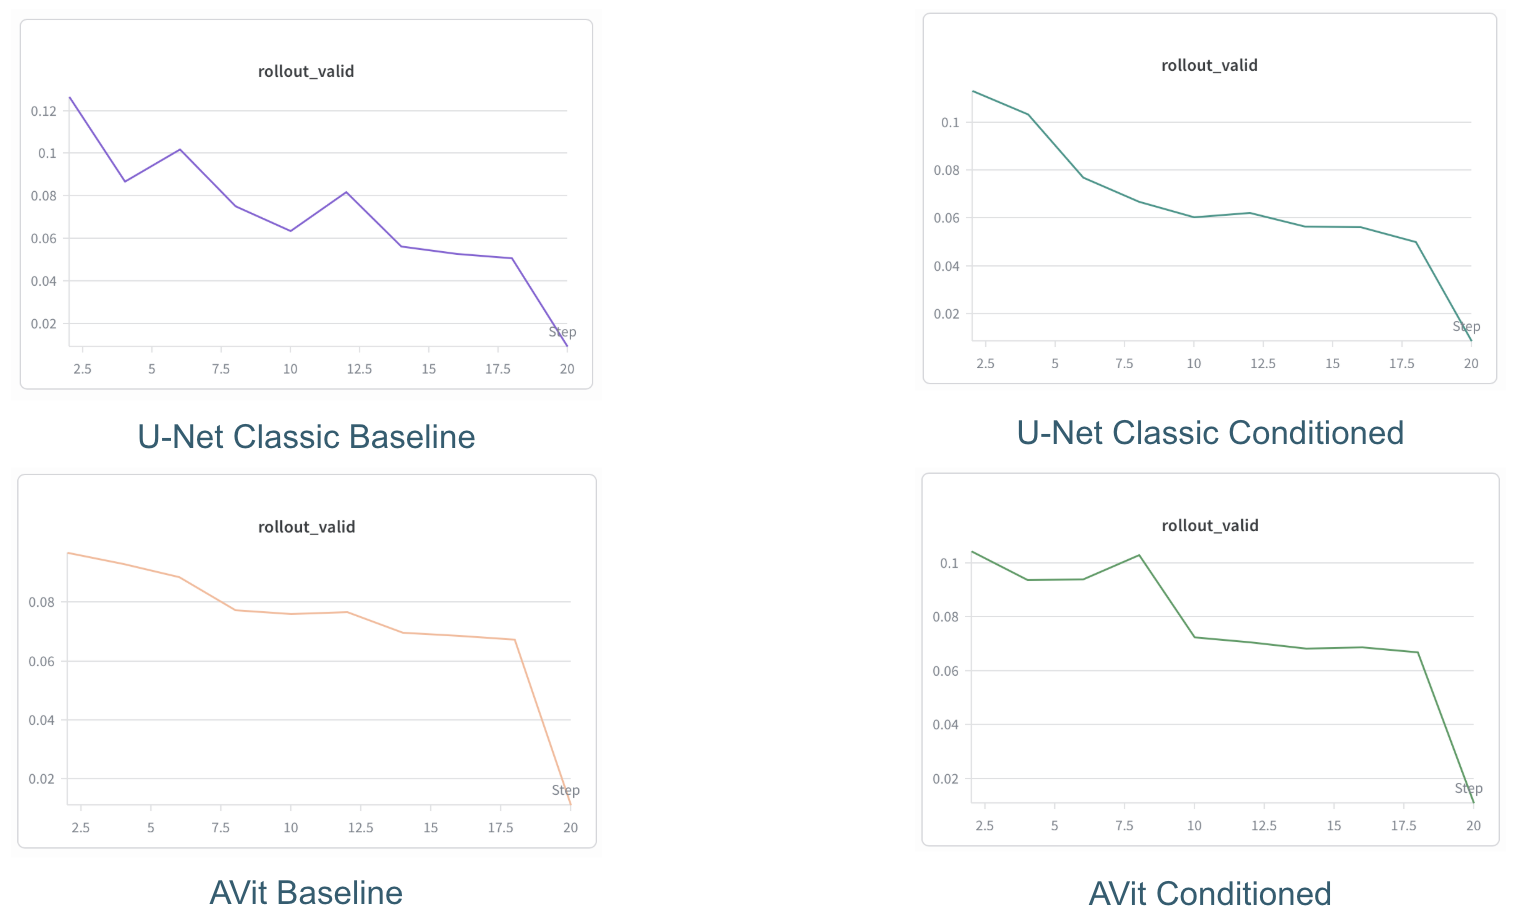
\includegraphics[width=0.9\columnwidth]{figures/rollout_loss.png}
\caption{Rollout loss comparison}
\label{fig:rollout}
\end{figure}

\subsection{Detailed Metrics}

\begin{table*}[t]
\centering
\caption{Detailed Performance Metrics}
\begin{tabular}{lcccc}
\hline
Model & Loss & MSE & RMSE & $L_\infty$ \\
\hline
UNetClassic & 0.13623 & 0.00096 & 0.03091 & 0.18391 \\
UNetConditioned & 0.13802 & 0.00637 & 0.07981 & 0.23783 \\
AViT & 0.48020 & 0.18382 & 0.40078 & 1.48433 \\
\hline
\end{tabular}
\end{table*}

% (Continue rest of analysis)

\section{Conclusion}

% (Paste conclusion)

\bibliographystyle{iclr2026_conference}
\bibliography{references}

\end{document}